\documentclass[12pt]{article}

\usepackage[margin=1in]{geometry}
\usepackage{amsmath, amssymb} 
\usepackage{graphicx} 

\title{Face Recognition using Principal Component Analysis}
\author{Darsh Raghuvanshi - 25B2224}

\begin{document}
\maketitle

\section{Introduction}
The primary goal of this project is to implement a memory-efficient facial recognition system using linear algebra techniques. Specifically, we utilize Principal Component Analysis (PCA), a dimensionality reduction algorithm that transforms a large, high-dimensional dataset into a smaller set of orthogonal variables called principal components. By extracting these components from a dataset of human faces, we generate "Eigenfaces" (a concept by Turk and Pentland). These Eigenfaces represent the core characteristic features of the dataset, allowing the system to recognize individuals by calculating how their specific face projects onto these key features, rather than attempting to compare every single raw pixel

\subsection{The Dataset}
The dataset used is the ORL Database of Faces. It consists of $M = 400$ grayscale images belonging to 40 different individuals (10 images per person). Each image has a resolution of $112 \times 92$ pixels.

\section{Mathematical Framework}

\subsection{Image Flattening and Vectorization}
In order to apply PCA, each 2D image matrix must be flattened into a 1D column vector. Given an image of size $r \times c$, the flattened vector $x_i$ has a dimension of $L = r \times c$. For this dataset, $L = 112 \times 92 = 10,304$. 

The entire dataset can be represented as an $L \times M$ matrix $A$:
\begin{equation}
    A = [x_1, x_2, \dots, x_M]
\end{equation}

\subsection{Mean Subtraction}
Before calculating the covariance, the dataset must be centered by subtracting the ``mean face'' ($\mu$) from every image vector.
\begin{equation}
    \mu = \frac{1}{M} \sum_{i=1}^{M} x_i
\end{equation}
The mean-centered data matrix $C$ is then calculated as:
\begin{equation}
    C = [x_1 - \mu, x_2 - \mu, \dots, x_M - \mu]
\end{equation}
Subtracting the mean face from every individual image is a crucial preprocessing step in PCA. It mathematically centers the dataset around the origin without altering the relative distances between the data points. By ensuring the data has a mean of zero, the subsequent covariance matrix will accurately capture the directions of maximum variance, meaning it will map how the faces differ from the average face.

\subsection{Covariance and Eigenfaces}
The covariance matrix $S$ of the mean-centered data is given by:
\begin{equation}
    S = C \cdot C^T
\end{equation}
By performing eigen decomposition on $S$, we obtain a set of eigenvectors and eigenvalues. The eigenvectors corresponding to the largest eigenvalues represent the directions of maximum variance in the data. In the context of facial images, these eigenvectors are referred to as \textbf{Eigenfaces}.

\section{Code Implementation and Methodology}
\subsection{Data Preprocessing}
The dataset is distributed as a compressed archive. To efficiently process this without manual extraction, the zipfile library is utilized to iterate directly through the archive. Each valid image file is read as a byte string and immediately decoded into a 2D NumPy array using OpenCV (\texttt{cv2.imdecode} with the \texttt{cv2.IMREAD\_GRAYSCALE} flag). To properly evaluate the model's accuracy, the dataset is deliberately split: pictures of 39 individuals are flattened and stored in a 2D NumPy array (\texttt{facematrix}) for training, while specific images, such as image 10 of subject 39, is intentionally held out as an out of sample test set.

\subsection{Applying PCA}
Rather than computing the covariance matrix and solving for eigenvectors manually, the implementation relies on \texttt{PCA().fit(facematrix)} function from the scikit-learn library. The algorithm identifies the principal components, and for this project, we keep only the top 50 components (n\_components = 50). This represents a massive degree of data compression: an original face requiring 10,304 individual pixel values is compressed into a numerical vector of just 50 mathematical weights, while still retaining enough critical facial geometry to successfully identify the subject.

\subsection{Projecting Data onto Eigenfaces (Weights)}
Once the top $K$ eigenfaces are extracted, the original mean-subtracted faces are projected onto this new subspace to find their weights:
\begin{equation}
    W = F \cdot C^T
\end{equation}
Where $F$ is the matrix of Eigenfaces. 
To convert the original high-dimensional faces into our new, compressed 50-dimensional space, we project the mean-centered training data onto the Eigenfaces matrix. In the code, this is executed via the line \texttt{weights = eigenfaces @ (facematrix - pca.mean\_).T} (line 59). The @ symbol is Python's dedicated operator for matrix multiplication. This operation yields a specific weight vector for each training image, detailing exactly what proportion of each Eigenface is required to successfully reconstruct that specific person's face.

\section{Face Recognition Process}
\subsection{Testing and Euclidean Distance}
To recognize an unknown face, the test image is first flattened, mean-centered, and projected onto the eigenfaces to generate its specific weight vector ($\omega_{test}$). 

The system then calculates the Euclidean distance between this test weight vector and all known training weight vectors ($\omega_{train}$):
\begin{equation}
    d_i = \|\omega_{test} - \omega_{train, i}\|_2
\end{equation}
The code utilizes NumPy's \texttt{np.linalg.norm} function (line 65) to calculate the L2 norm, or Euclidean distance, between the test image's vector and the vectors of the training images. A smaller mathematical distance indicates a higher visual similarity in the compressed subspace. The training image index that yields the absolute lowest distance is located using \texttt{np.argmin()} (line 66) and is declared the Best Match by the algorithm.

\section{Results and Conclusion}
Visualizing the results confirms the effectiveness of the Eigenface approach. When plotting the query image alongside the system's calculated "Best Match," the model successfully identifies the correct individual from the training set, despite the test image being previously unseen. PCA proves to be an incredibly memory-efficient method for facial recognition, successfully reducing dataset complexity by over 99 percent (from 10,304 dimensions to just 50). However, it should be noted that traditional Eigenface models are highly sensitive to extreme variations in lighting, facial expressions, and head poses, which can alter the principal components and occasionally lead to misclassification.

\begin{figure}[h]
     \centering
     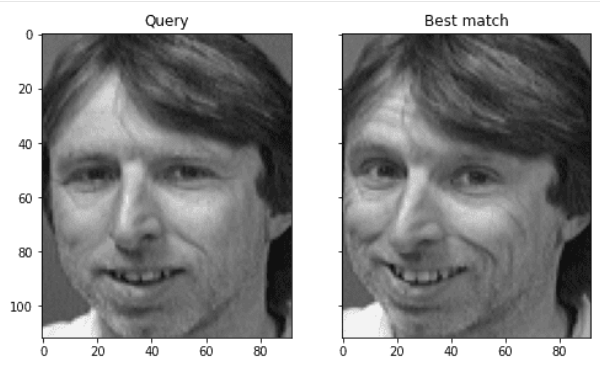
\includegraphics[width=0.7\textwidth]{Subject_39_image_10.png}
     \caption{Query face compared to the Best Match identified by the algorithm.}
     \label{fig:match1}
\end{figure}

\begin{figure}[h]
     \centering
     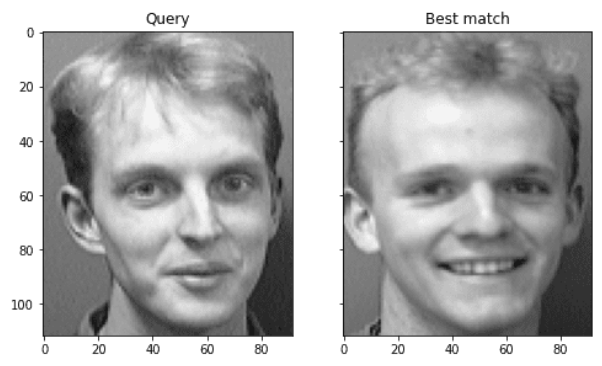
\includegraphics[width=0.7\textwidth]{Subject_40.png}
     \caption{New face held out of PCA as query identified by the algorithm.}
     \label{fig:match2}
\end{figure}

\end{document}
